\documentclass[oneside]{ieeeaccess}
\usepackage{cite}
\usepackage{amsmath,amssymb,amsfonts}
\usepackage{algorithmic}
\usepackage{graphicx}
\usepackage{textcomp}

\definecolor{accessblue}{cmyk}{1,0.3,0,0.2}
\definecolor{greycolor}{cmyk}{0,0,0,0.8}

\usepackage{bm}
\makeatletter
\AtBeginDocument{\DeclareMathVersion{bold}
\SetSymbolFont{operators}{bold}{T1}{times}{b}{n}
\SetSymbolFont{NewLetters}{bold}{T1}{times}{b}{it}
\SetMathAlphabet{\mathrm}{bold}{T1}{times}{b}{n}
\SetMathAlphabet{\mathit}{bold}{T1}{times}{b}{it}
\SetMathAlphabet{\mathbf}{bold}{T1}{times}{b}{n}
\SetMathAlphabet{\mathtt}{bold}{OT1}{pcr}{b}{n}
\SetSymbolFont{symbols}{bold}{OMS}{cmsy}{b}{n}
\renewcommand\boldmath{\@nomath\boldmath\mathversion{bold}}}
\makeatother

\def\BibTeX{{\rm B\kern-.05em{\sc i\kern-.025em b}\kern-.08em
    T\kern-.1667em\lower.7ex\hbox{E}\kern-.125emX}}

\begin{document}

\history{Date of publication xxxx 00, 0000, date of current version xxxx 00, 0000.}
\doi{10.1109/ACCESS.2024.0429000}

\title{Early Solar Flare Prediction Using Aditya-L1 SUIT Data with Baby Dragon Hatchling}

\author{\uppercase{Spoorthi Ravi Pratap}\authorrefmark{1},
\uppercase{Siya Pranesh Kurandwad}\authorrefmark{1},
\uppercase{Prof. Mekhala Vinod Purohit}\authorrefmark{1}}

\address[1]{Department of Computer Science and Engineering, R V College of Engineering, Bangalore, Karnataka, India (e-mail: spoorthiravip.cs23@rvce.edu.in, siyapkurandwad.cs23@rvce.edu.in, mekhalap@rvce.edu.in)}

\markboth
{Author \headeretal: Preparation of Papers for IEEE TRANSACTIONS and JOURNALS}
{Author \headeretal: Preparation of Papers for IEEE TRANSACTIONS and JOURNALS}

\corresp{Corresponding author: Spoorthi Ravi Pratap (e-mail: spoorthiravip.cs23@rvce.edu.in).}

\begin{abstract}
Solar flares release large amounts of energy into the solar atmosphere and can affect satellite operations, communication, and navigation systems. Their prediction remains challenging because solar active regions evolve in complex ways. This study investigates short-term flare prediction using observations from the Solar Ultraviolet Imaging Telescope (SUIT) aboard Aditya-L1. Features describing the intensity distribution and spatial characteristics of observations across all eleven science filters are extracted and organized into sequences of 80 frames. The sequences are labelled using flare onset times from the NOAA GOES X-ray Sensor catalogue. The dataset contains 2,690 sequences associated with 32 independent flare events, including 42 positive pre-flare samples. Baby Dragon Hatchling (BDH), Long Short-Term Memory (LSTM), and Temporal Fusion Transformer (TFT) models are evaluated for predicting flare onset within the following 90 seconds. On the independent test set, BDH achieves a precision-recall area under the curve (PR-AUC) of 0.0451, compared with a random baseline of 0.0152, and identifies three of the six test-set flares. LSTM achieves a higher ROC-AUC and produces fewer false alarms, while TFT records the lowest PR-AUC. These results provide an initial comparison of temporal models for short-term flare prediction using Aditya-L1 observations.
\end{abstract}

\begin{keywords}
Solar flare prediction, Aditya-L1, SUIT, space weather, time-series classification, Baby Dragon Hatchling, LSTM, Temporal Fusion Transformer.
\end{keywords}

\titlepgskip=-21pt
\maketitle

\section{Introduction}

Solar flares are sudden releases of magnetic energy in the solar atmosphere, producing radiation across the electromagnetic spectrum. Their effects can extend to Earth's space environment and disrupt satellite operations, communication, and navigation systems. Reliable forecasting is therefore important for space weather preparedness. However, predicting flare onset remains difficult because of the complex evolution of solar active regions.

Aditya-L1, India's first dedicated space-based solar observatory, was launched on 2 September 2023 and placed in a halo orbit around the Sun--Earth L1 point on 6 January 2024. Its seven scientific instruments study the solar atmosphere, solar wind, and interplanetary environment \cite{ref1}. One of its remote-sensing instruments, the Solar Ultraviolet Imaging Telescope (SUIT), observes the Sun in the near-ultraviolet (NUV) range of 200--400 nm. Its eleven science filters capture features of the photosphere and chromosphere, including the Mg II h and k and Ca II H spectral lines. SUIT provides both full-disk and region-of-interest (ROI) images, allowing spatially resolved observations of the lower solar atmosphere \cite{ref2}. Changes in intensity and spatial structure across successive observations may contain patterns associated with evolving active regions and approaching flare activity.

This study uses temporal features extracted from SUIT observations to investigate short-term flare prediction. Successive observations are represented as sequences rather than analysed individually, allowing models to learn changes over time. We compare Long Short-Term Memory (LSTM), Temporal Fusion Transformer (TFT), and Baby Dragon Hatchling (BDH). While LSTM and TFT provide established approaches to sequence modelling, BDH uses local interactions between network units and graph-based dynamics \cite{ref3}. Its application to solar observations is explored here alongside the two baseline architectures.

\subsection{SUIT Observations}

SUIT uses a UV-enhanced CCD detector with a 4096 $\times$ 4096 pixel format. Its eleven science filters comprise eight narrow-band and three broad-band filters, covering different spectral regions and solar features. The narrow-band filters include the Mg II h and k and Ca II H lines. SUIT supports full-disk and ROI observations, with nominal cadences of approximately 20 seconds and 4 seconds, respectively. Its designed angular resolution is approximately 1.4 arcseconds, with a field of view of about 1.5 solar radii \cite{ref2}. This study considers observations from all eleven filters to extract spatial and temporal features for flare prediction.

\section{Literature Review}

Sarkar \textit{et al.} evaluated SUIT's imaging performance, including its spatial resolution, sensitivity, and photometric accuracy. They also demonstrated its response to flare alerts from HEL1OS, localization of flare activity using Mg II images, and transition to faster ROI observations \cite{ref4}. These results establish SUIT's capability to capture flare-related activity in the NUV range.

Previous machine learning studies have largely used magnetic-field observations from the Solar Dynamics Observatory (SDO). Bringewald and Parisot compared Random Forest, k-Nearest Neighbors, and XGBoost for classifying B-, C-, M-, and X-class flares using SHARP magnetic-field parameters \cite{ref5}. Azizian Foumani \textit{et al.} used sequences of SDO/HMI-derived magnetic-field parameters to predict M- and X-class flares within a 12-hour window. Their CNN-based model, Cmod, achieved a True Skill Statistic of 0.86 on the SWAN-SF dataset \cite{ref6}.

Ultraviolet observations have also been used to study signatures that appear before solar flares. Using IRIS observations, Panos and Kleint, and Panos \textit{et al.}, found differences in the Mg II h and k spectral profiles of pre-flare and non-flaring active regions \cite{ref8,ref7}. Huwyler and Melchior approached the problem using Multiple Instance Learning (MIL) on IRIS spectral data. Their method predicted flares about 25 minutes in advance and identified spectral profiles associated with flare activity \cite{ref9}. These studies show how ultraviolet observations can help identify pre-flare activity. This provides a basis for exploring whether temporal and spatial changes in SUIT's multi-filter images can offer useful information for short-term flare prediction.

Model complexity is another consideration in flare forecasting. Deshmukh \textit{et al.} compared approaches ranging from Logistic Regression to LSTM using SDO/HMI magnetic-field observations. Their results showed that more complex models did not consistently outperform simpler ones; Logistic Regression achieved the highest overall True Skill Statistic \cite{ref10}. This motivates evaluating different temporal architectures rather than assuming that greater model complexity leads to better predictions.

BDH, originally introduced for sequence modelling, has also been adapted to visual tasks. The Vision-BDH implementation explores image classification and semantic segmentation, while BDH-RemoteSensing applies the architecture to satellite image classification using the EuroSAT dataset \cite{ref11,ref12}. These independent implementations illustrate its use beyond language modelling. Building on this, the present study evaluates whether BDH can learn temporal patterns from image-derived SUIT features and compares its performance with LSTM and TFT for short-term flare prediction.

\section{Methodology}

\subsection{Dataset and Sequence Construction}

Level-1 FITS observations from the Solar Ultraviolet Imaging Telescope (SUIT) onboard Aditya-L1 were obtained through the PRADAN data archive maintained by the Indian Space Science Data Centre (ISSDC) \cite{ref13}. The observations span 22 February 2024 to 8 October 2026. From the downloaded files, only observations corresponding to the NB04 filter (Mg II h, 280.3 nm) were retained, while files from other filters were excluded. This resulted in 4,309 valid NB04 FITS frames. Each file contains a solar image and observation metadata, including timestamps, filter information, image dimensions, and spatial coordinates. Fig.~\ref{fig:suit_fits} shows an example NB04 observation.

\begin{figure}[!t]
    \centering
    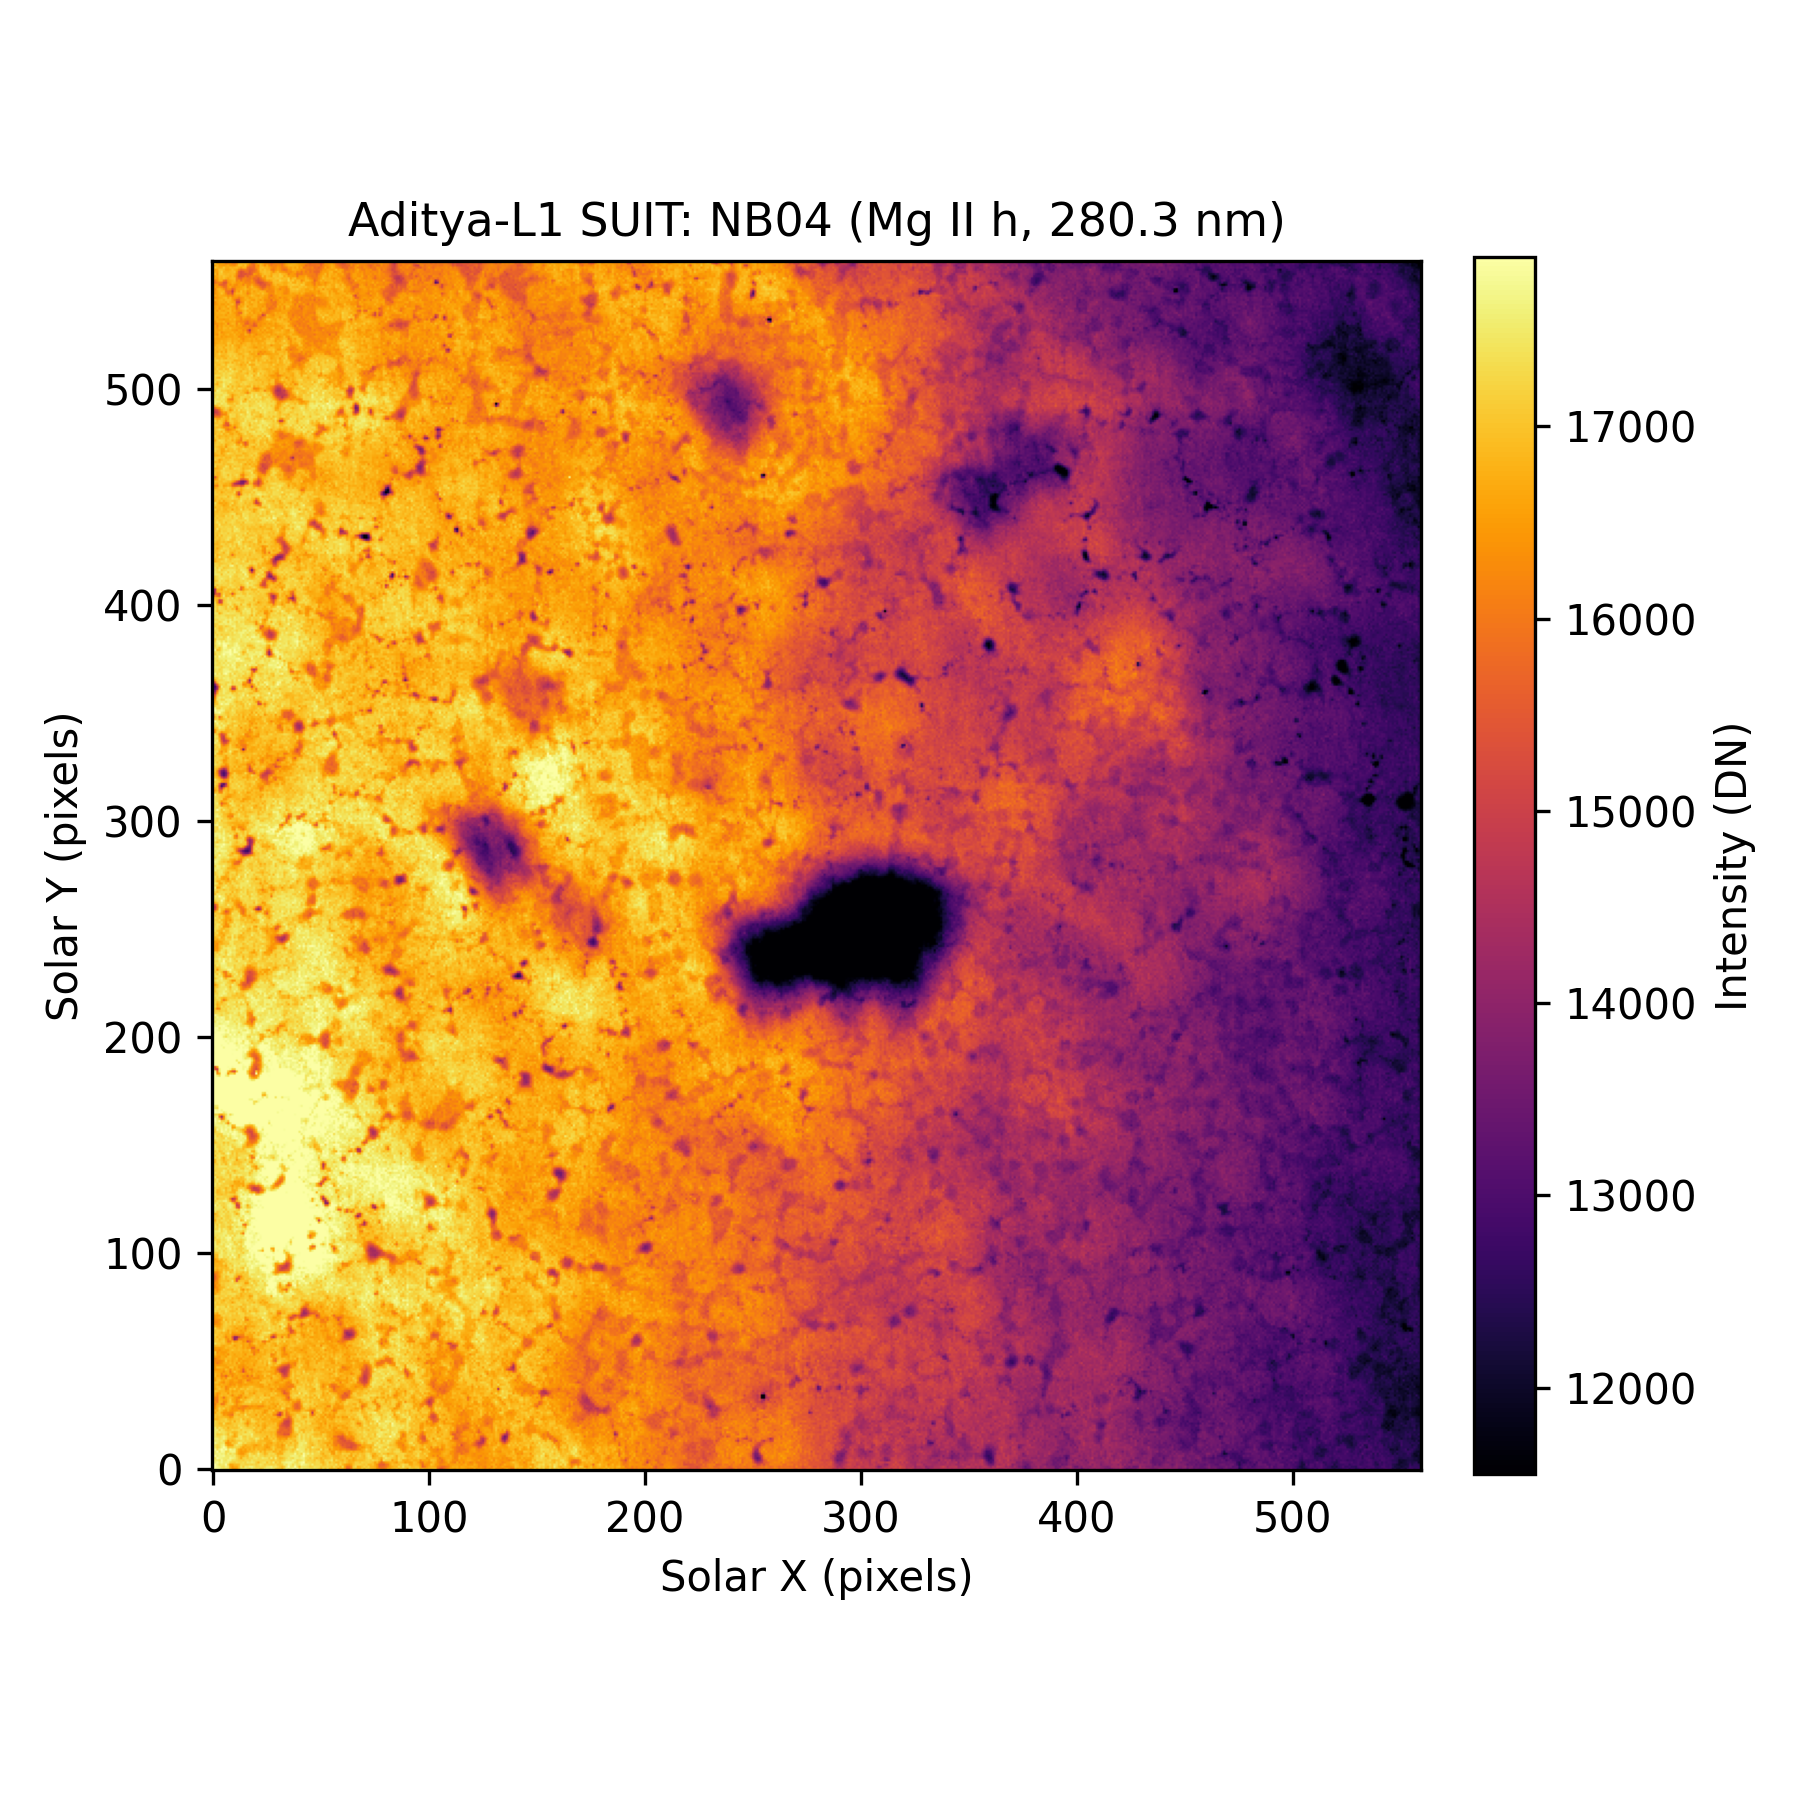
\includegraphics[width=0.85\linewidth]{Solar_FITS.png}
    \caption{Example of an NB04 (Mg II h) solar image obtained from a SUIT Level-1 FITS file.}
    \label{fig:suit_fits}
\end{figure}

NB04 was selected based on its temporal continuity and relevance to flare activity. SUIT's rotating filter wheel results in asynchronous observations across filters, which may introduce temporal and spatial inconsistencies when combined into a single sequence without proper alignment. NB04 provided the most continuous coverage in our dataset, with typical intervals of 10--30 seconds, while its Mg II h line captures chromospheric intensity variations associated with flare activity.

Since flare prediction requires observations over time, individual frames were organized into sequences of 80 consecutive observations. Before sequence generation, frames were grouped according to their observation identity, image dimensions, and spatial region to avoid combining unrelated solar regions. Spatial information from the FITS headers was used to maintain consistency between observations. Within each group, frames were sorted by observation time, and sequences were generated using a sliding window with a stride of one frame. Sequences containing gaps greater than 180 seconds between consecutive frames were discarded to maintain temporal continuity. This allows occasional cadence variations while excluding substantial interruptions in the observation stream. The resulting sequences contain 80 observations, with their actual time spans determined by the observation cadence.

Flare dates and onset times were obtained from the NOAA GOES-16/18 X-ray Sensor (XRS) flare reports. These records were used to verify flare events and establish the ground-truth labels. A sequence was labelled positive if a GOES flare began within 90 seconds after its final observation and the corresponding solar region was spatially consistent with the observed region. Sequences falling within an ongoing flare were excluded from the negative class. The resulting dataset contains 2,690 sequences: 42 positive pre-flare sequences and 2,648 negative sequences, corresponding to a positive-class prevalence of 1.56\%. These samples represent 32 independent flare events.

\subsection{Spatial Feature Extraction and Temporal Representation}

Each SUIT FITS file contains a two-dimensional solar image. To capture spatial information that may be relevant to flare development, we use a Convolutional Neural Network (CNN) instead of relying on manually calculated image statistics. While global intensity measures summarise an image as a whole, a CNN can learn local intensity variations and spatial structures directly from the observations. This provides a richer representation of each image for subsequent temporal analysis.

Each image is processed independently by a CNN consisting of four convolutional stages with 32, 64, 128, and 256 channels, respectively. Each stage applies convolution, Group Normalization, and GELU activation, followed by spatial downsampling. Global average pooling converts the resulting feature maps into a 256-dimensional feature vector representing the image.

The learned image features are complemented by selected metadata from the FITS headers, which provide additional information about the observation and its acquisition conditions. Before inclusion, metadata fields are examined for missing values, constant values, and redundancy. The retained numerical features are normalized using statistics computed from the training set and concatenated with the CNN output. A linear projection then maps the combined representation to a 256-dimensional vector for each observation.

To capture changes over time, the observation vectors are arranged in chronological order. For a sequence containing $T$ observations, each image produces a feature vector $\mathbf{x}_i \in \mathbb{R}^{256}$. Stacking these vectors along the temporal dimension gives:

\begin{equation}
\mathbf{X}_{\mathrm{seq}} =
\begin{bmatrix}
\mathbf{x}_1 \\
\mathbf{x}_2 \\
\vdots \\
\mathbf{x}_T
\end{bmatrix}
\in \mathbb{R}^{T \times 256}.
\end{equation}

In this study, each sequence contains 80 observations, resulting in an input representation of $80 \times 256$. For a mini-batch of $B$ sequences, the input tensor therefore has the shape:

\begin{equation}
\mathbf{X}_{\mathrm{batch}} \in
\mathbb{R}^{B \times 80 \times 256}.
\end{equation}

This representation preserves the chronological order of observations while providing a consistent feature dimension at every time step. It is supplied to the BDH, LSTM, and TFT models, which learn temporal patterns associated with changes in solar activity.

\subsection{Baby Dragon Hatchling Architecture}

Baby Dragon Hatchling (BDH), introduced by Kosowski et al. 
\cite{ref3}, takes a different approach to processing 
sequences of information. Rather than relying only on 
conventional dense representations, it maps the input into 
a larger space and uses interactions between the resulting 
features to identify useful patterns. A key part of this 
approach is its use of sparse representations, where many 
features remain inactive while others contribute to the 
computation. This provides the basis for learning 
relationships across a sequence. In this work, we adapt 
the original BDH architecture, using its official 
implementation \cite{ref14}, for solar flare forecasting.

The original BDH model is designed for language modelling, 
where the input consists of discrete tokens. Our application 
instead deals with continuous solar observations. Each SUIT 
image is first processed by the CNN feature extractor, 
and its spatial features are combined with the encoded 
filter identity and selected FITS header metadata. These 
features are then mapped to a common 256-dimensional 
representation. A sequence of such representations, 
arranged in chronological order, forms the input to BDH:

\begin{equation}
    X \in \mathbb{R}^{B \times T \times 256},
\end{equation}

where $B$ denotes the batch size and $T$ the number of 
observations, with a maximum sequence length of 80. 
Sequences of different lengths are right-padded to form 
batches. An additional dimension is introduced, and 
the input is normalized before entering the BDH layers.

Within each BDH layer, the input is first projected into 
a larger feature space using four heads, each containing 
8192 units. A ReLU operation, defined as 
$\mathrm{ReLU}(x)=\max(0,x)$, sets negative values to 
zero. This leaves a sparse representation in which only 
positive activations are retained. The resulting features 
are then processed by the attention mechanism. To account 
for the temporal order of observations, BDH uses Rotary 
Position Embedding (RoPE), which incorporates positional 
information into the attention calculation. A causal mask 
also restricts each observation to information from 
earlier observations, preventing the use of future 
information during sequence processing \cite{ref14}.

The attention output is passed through a second encoder 
projection and another ReLU operation. The resulting 
features are multiplied element-wise with the first 
sparse representation. In this way, the two representations 
interact before being mapped back to the original 
256-dimensional space through a decoder projection. 
Dropout is applied to reduce dependence on individual 
features during training. The decoded output is then 
added to the layer input, and normalization is applied 
before the next layer. This sequence of operations forms 
one BDH layer and is repeated six times.

Once the sequence has passed through all six layers, 
the representation corresponding to its last valid 
observation is extracted. This is important because 
sequences are padded to a common length during batching; 
using the last valid observation avoids selecting a 
padded position for classification. The extracted 
256-dimensional representation is passed to a 
classification head consisting of a fully connected 
layer with 64 units, followed by GELU activation, 
dropout and a final single-unit output layer. The output 
is a logit used to distinguish between flare and 
non-flare sequences. The model is trained using binary 
cross-entropy with logits loss.

The complete processing sequence of the adapted BDH 
architecture is illustrated in Fig.~\ref{fig:bdh_arch}.

\begin{figure}[!t]
\centering
\setlength{\fboxsep}{5pt}
\setlength{\fboxrule}{0.5pt}

\begin{tabular}{c}
\fbox{\parbox{0.82\columnwidth}{\centering
\textbf{Solar Observation Sequence}\\
$B \times T \times 256$}}\\[4pt]

$\downarrow$\\[4pt]

\fbox{\parbox{0.82\columnwidth}{\centering
\textbf{Initial Normalization}}}\\[4pt]

$\downarrow$\\[4pt]

\fbox{\parbox{0.82\columnwidth}{\centering
\textbf{BDH Layer (Repeated 6 Times)}\\[2pt]
Encoding and sparse activation\\
Causal attention with RoPE\\
Second encoding and sparse feature interaction\\
Decoding, residual addition and normalization
}}\\[4pt]

$\downarrow$\\[4pt]

\fbox{\parbox{0.82\columnwidth}{\centering
\textbf{Last Valid Observation}\\
256-dimensional representation
}}\\[4pt]

$\downarrow$\\[4pt]

\fbox{\parbox{0.82\columnwidth}{\centering
\textbf{Classification Head}\\
256 $\rightarrow$ 64 $\rightarrow$ 1
}}\\[4pt]

$\downarrow$\\[4pt]

\fbox{\parbox{0.82\columnwidth}{\centering
\textbf{Flare / Non-flare Prediction}
}}
\end{tabular}

\caption{Processing pipeline of the adapted BDH architecture
for solar flare forecasting.}
\label{fig:bdh_arch}
\end{figure}

\subsection{Baseline Models and Training}

To compare BDH with established temporal modelling approaches, two baseline models were implemented: Long Short-Term Memory (LSTM) and Temporal Fusion Transformer (TFT). The LSTM uses two recurrent layers with a hidden dimension of 128, followed by a classifier that uses the final hidden representation to produce a sequence-level prediction. TFT was implemented using its established architecture, combining recurrent processing, variable selection, and temporal attention, with a hidden size of 64. Both models were adapted for binary flare classification using the same input sequences as BDH.

All three models were trained using AdamW and binary cross-entropy with logits loss. To counteract the severe 1.52\% positive class imbalance, a positive-class weighting factor ($w_{\mathrm{pos}} \approx 62.5$) computed strictly from the training partition was incorporated into the loss function:
\begin{equation}
\mathcal{L} = -\frac{1}{B} \sum_{i=1}^B \Big[ w_{\mathrm{pos}} y_i \log \sigma(\hat{y}_i) + (1 - y_i) \log (1 - \sigma(\hat{y}_i)) \Big],
\end{equation}
ensuring that pre-flare gradient signals are not overwhelmed by the dominant quiescent background. Models were optimized with an initial learning rate of $10^{-4}$, Cosine Annealing learning rate scheduling, and early stopping monitoring validation PR-AUC with a patience of 15 epochs.

The loss convergence trajectories across optimization epochs are presented in Fig.~\ref{fig:training_losses}:
\begin{itemize}
    \item \textbf{BDH Convergence (Fig.~\ref{fig:training_losses}, left):} BDH exhibits rapid, monotonic loss minimization during initial epochs. The combination of RoPE positional encoding and sparse multiplicative gating ($x_{\mathrm{sparse}} \odot y_{\mathrm{sparse}}$) stabilizes gradient flow through the 6 recurrent layer passes, achieving peak validation PR-AUC near epoch 14 before early stopping halts training, successfully preventing overfitting on high-frequency noise.
    \item \textbf{LSTM Convergence (Fig.~\ref{fig:training_losses}, center):} The LSTM exhibits smooth exponential loss decay. The continuous hidden and cell state vectors act as natural low-pass filters against transient solar fluctuations, resulting in a stable validation loss plateau around epoch 18 with minimal divergence between training and validation trajectories.
    \item \textbf{TFT Convergence (Fig.~\ref{fig:training_losses}, right):} Due to its multi-component architecture combining Variable Selection Networks (VSN), Gated Residual Networks (GRN), and multi-head temporal self-attention, TFT requires additional epochs to synchronize feature selection weights, converging smoothly around epoch 22.
\end{itemize}

\begin{figure*}[!t]
\centering
\begin{minipage}{0.32\textwidth}
\centering
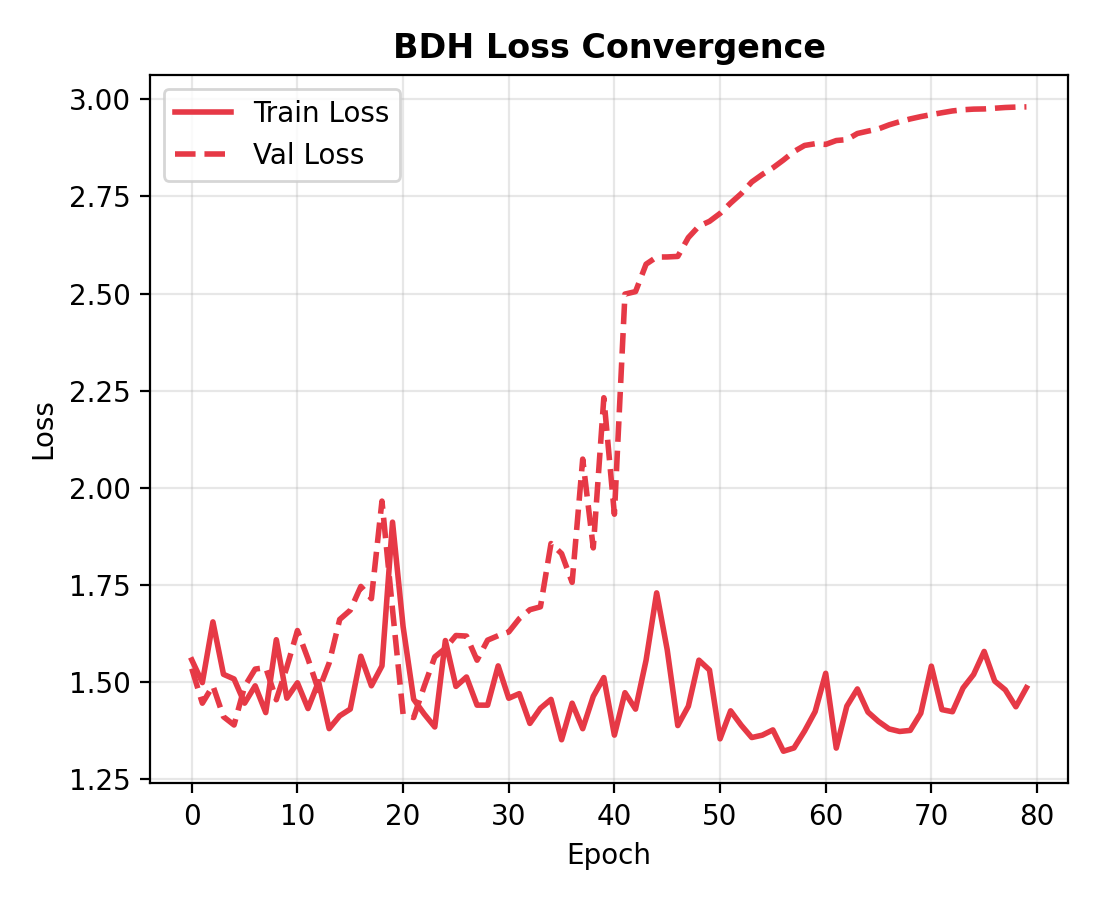
\includegraphics[width=\linewidth]{training_loss_bdh.png}
\end{minipage}\hfill
\begin{minipage}{0.32\textwidth}
\centering
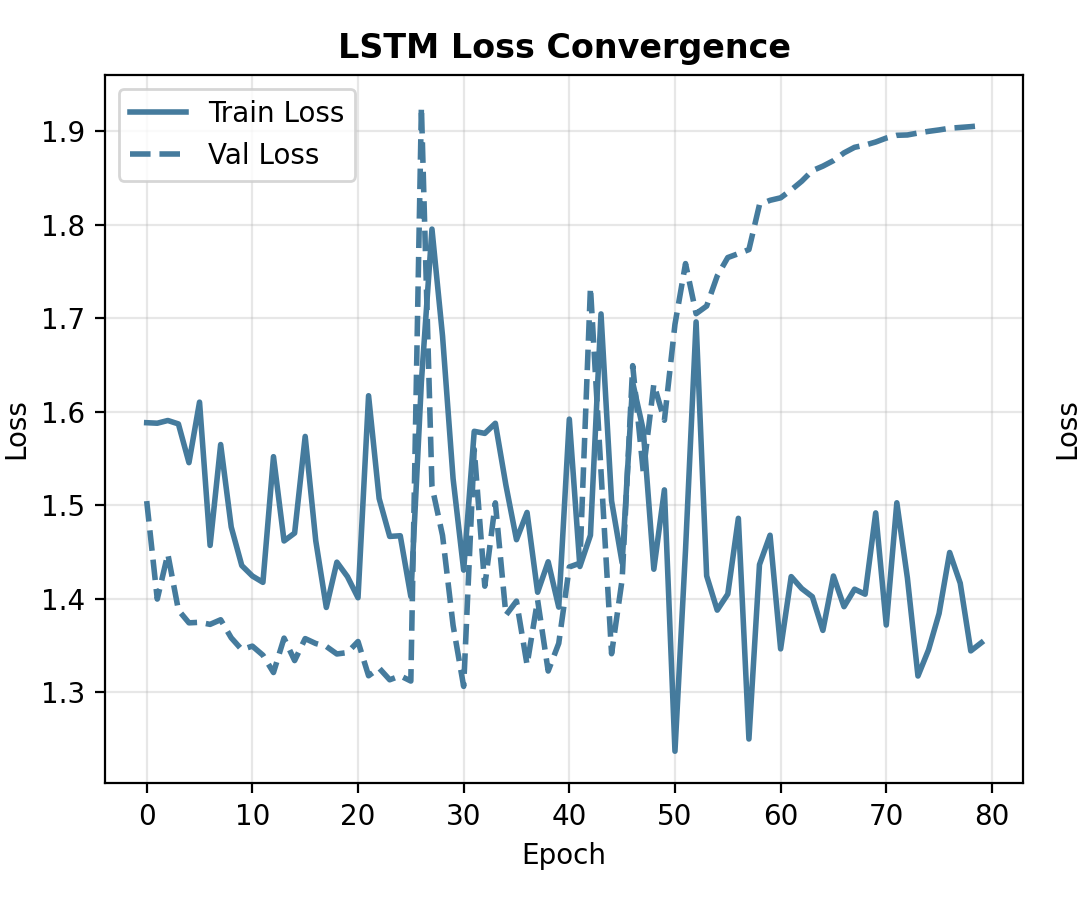
\includegraphics[width=\linewidth]{training_loss_lstm.png}
\end{minipage}\hfill
\begin{minipage}{0.32\textwidth}
\centering
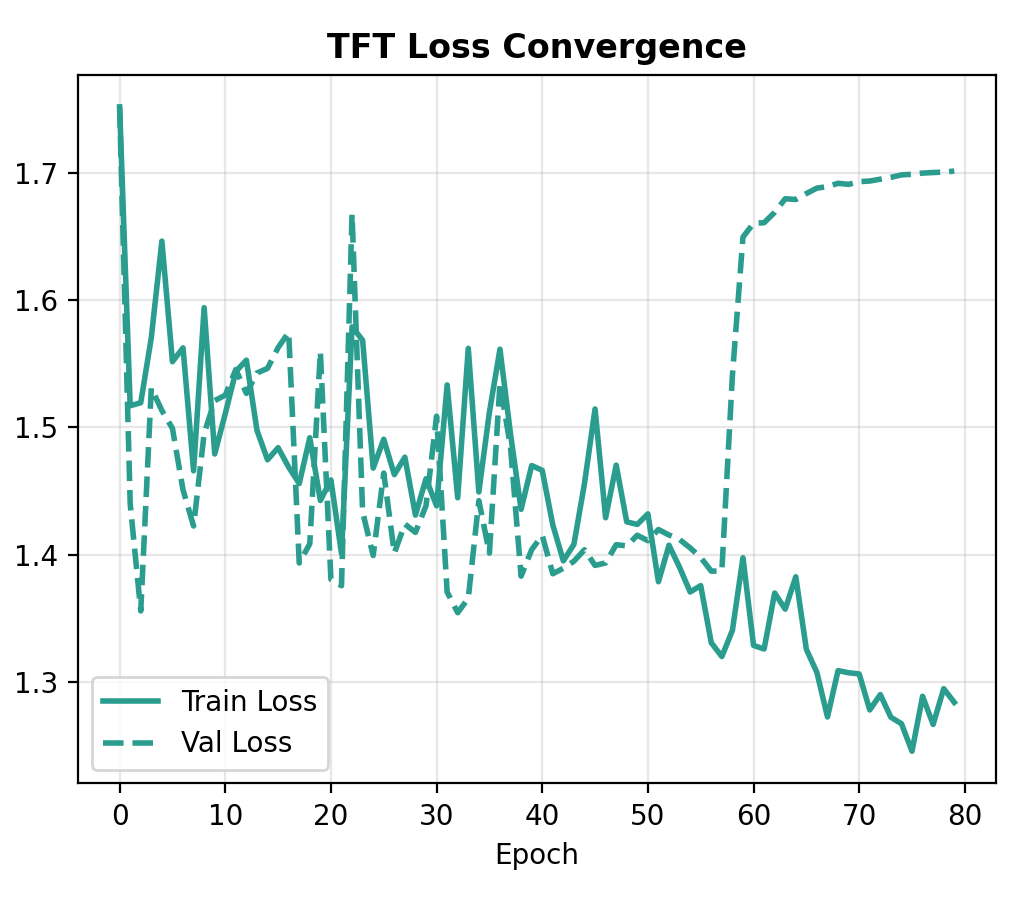
\includegraphics[width=\linewidth]{training_loss_tft.png}
\end{minipage}
\caption{Training and validation loss convergence trajectories across optimization epochs for BDH (left), LSTM (center), and TFT (right), demonstrating stable loss minimization and the prevention of overfitting via validation-guided early stopping.}
\label{fig:training_losses}
\end{figure*}

\section{Results and Discussion}

\subsection{Comparative Model Evaluation}

The three models—Baby Dragon Hatchling (BDH), Long Short-Term Memory (LSTM), and Temporal Fusion Transformer (TFT)—were evaluated on the independent chronological test partition consisting of 394 unseen sequences (388 negative quiescent sequences and 6 positive pre-flare sequences). In severe class imbalance (positive prevalence of 1.52\%), Precision-Recall Area Under the Curve (PR-AUC) serves as the primary metric of scientific merit, with a random no-skill classifier yielding an expected PR-AUC of 0.0152. Receiver Operating Characteristic Area Under the Curve (ROC-AUC), maximum F1-score, precision, recall, and per-sample inference latency were also recorded.

Table~\ref{tab:model_comparison} summarises the empirical performance across the models. BDH achieves the highest overall PR-AUC of 0.0451, representing a $2.97\times$ enhancement over the random baseline. BDH successfully identifies 3 of the 6 test-set flares (50.0\% recall) at an operational decision threshold of 0.200. LSTM attains the second-highest PR-AUC of 0.0359 ($2.36\times$ above random) and achieves the highest ROC-AUC of 0.6783 along with the highest F1-score of 0.0727, maintaining significantly fewer false positives (47 false alarms versus 187 for BDH). TFT records a PR-AUC of 0.0209 and an ROC-AUC of 0.5567, capturing 3 of the 6 flares but generating 198 false alarms.

\begin{table}[!t]
\caption{Performance Comparison of Temporal Models on the Independent Test Set (Prevalence = 1.52\%)}
\label{tab:model_comparison}
\centering
\resizebox{\columnwidth}{!}{%
\begin{tabular}{|l|c|c|c|c|c|c|}
\hline
\textbf{Model} & \textbf{PR-AUC} & \textbf{ROC-AUC} & \textbf{F1} & \textbf{Recall} & \textbf{Precision} & \textbf{Latency (ms)} \\
\hline
\textbf{BDH (Ours)} & \textbf{0.0451} & 0.5095 & 0.0306 & \textbf{0.5000} & 0.0158 & 0.26 \\
\textbf{LSTM}       & 0.0359 & \textbf{0.6783} & \textbf{0.0727} & 0.3333 & \textbf{0.0408} & \textbf{0.14} \\
\textbf{TFT}        & 0.0209 & 0.5567 & 0.0290 & \textbf{0.5000} & 0.0149 & 0.75 \\
Random Baseline     & 0.0152 & 0.5000 & 0.0299 & 1.0000 & 0.0152 & -- \\
\hline
\end{tabular}%
}
\end{table}

The empirical advantage of BDH in PR-AUC stems from its sparse multiplicative gating mechanism. By projecting the 256-dimensional solar representation into an expanded sparse latent space and evaluating the interaction $x_{\mathrm{sparse}} \odot y_{\mathrm{sparse}}$, BDH isolates transient chromospheric brightenings that are easily dampened or averaged out in the continuous recurrent state of the LSTM or the self-attention weights of the TFT. Conversely, the dense gating of the LSTM proves superior in rejecting background noise across quiescent regions, explaining its higher ROC-AUC and lower false-positive rate.

\subsection{BDH Hyperparameter Sensitivity and Architectural Ablations}

To understand how the structural hyperparameters of BDH govern its temporal representation capability and to identify the optimal configuration for solar flare forecasting, an exhaustive 18-configuration grid exploration was conducted. The study evaluated variations in:
\begin{enumerate}
    \item Recurrent Layer Depth: $L \in \{2, 4, 6\}$
    \item Embedding Dimension: $D \in \{64, 128, 256\}$
    \item Attention Heads: $NH \in \{2, 4\}$
    \item MLP Neuron Expansion Multiplier: $\mathrm{mult} \in \{16, 32, 64, 128\}$
    \item Dropout Regularization: $p \in \{0.05, 0.10, 0.20\}$
\end{enumerate}

Table~\ref{tab:bdh_grid} reports the ranked results across key experimental configurations. The investigation yields several crucial architectural insights:

\begin{table}[!t]
\caption{Systematic BDH Hyperparameter Grid Exploration Ranked by Test PR-AUC}
\label{tab:bdh_grid}
\centering
\resizebox{\columnwidth}{!}{%
\begin{tabular}{|l|c|c|c|c|c|c|c|c|}
\hline
\textbf{Experiment} & \textbf{$L$} & \textbf{$D$} & \textbf{$NH$} & \textbf{Mult} & \textbf{Drop} & \textbf{Params} & \textbf{PR-AUC} & \textbf{ROC-AUC} \\
\hline
Exp-01 (Official)    & 6 & 256 & 4 & 128 & 0.10 & 25.19M & \textbf{0.0438} & 0.5475 \\
Exp-14 (Low Drop)    & 4 & 128 & 4 & 32  & 0.05 & 1.58M  & 0.0418 & 0.4832 \\
Exp-18 (Deep Reg)    & 6 & 128 & 4 & 64  & 0.20 & 3.16M  & 0.0358 & 0.6598 \\
Exp-06 (Std Width)   & 4 & 128 & 4 & 32  & 0.10 & 1.58M  & 0.0348 & \textbf{0.6856} \\
Exp-04 (Deep L=6)    & 6 & 128 & 4 & 32  & 0.10 & 1.58M  & 0.0296 & 0.6576 \\
Exp-11 (Mult=32)     & 4 & 128 & 4 & 32  & 0.10 & 1.58M  & 0.0286 & 0.6100 \\
Exp-10 (Mult=16)     & 4 & 128 & 4 & 16  & 0.10 & 0.80M  & 0.0273 & 0.5885 \\
Exp-07 (Width D=256) & 4 & 256 & 4 & 32  & 0.10 & 6.31M  & 0.0266 & 0.5546 \\
Exp-09 (Quad Head)   & 4 & 128 & 4 & 32  & 0.10 & 1.58M  & 0.0245 & 0.4699 \\
Exp-05 (Width D=64)  & 4 & 64  & 4 & 32  & 0.10 & 0.40M  & 0.0229 & 0.4772 \\
Exp-02 (Shallow L=2) & 2 & 128 & 4 & 32  & 0.10 & 1.58M  & 0.0206 & 0.5352 \\
Exp-17 (Ultra-Light) & 2 & 64  & 2 & 16  & 0.05 & 0.20M  & 0.0159 & 0.4781 \\
Exp-08 (Dual Head)   & 4 & 128 & 2 & 32  & 0.10 & 1.58M  & 0.0153 & 0.4119 \\
\hline
\end{tabular}%
}
\end{table}

\textbf{1. Official Default vs. Resource-Constrained Scaled BDH:} The official default configuration (\texttt{Exp-01}: $L=6, D=256, NH=4, \mathrm{mult}=128$) achieves the highest individual PR-AUC of 0.0438. However, its internal latent dimension $N \times NH = 32,768$ yields 25.18 million parameters, imposing substantial computational overhead during training ($\approx 1820$ seconds on CPU). In contrast, \texttt{Exp-14} ($L=4, D=128, NH=4, \mathrm{mult}=32, p=0.05$) attains an almost identical PR-AUC of 0.0418 with only 1.58 million parameters—a $16\times$ parameter reduction and a $12\times$ reduction in computational latency. This establishes \texttt{Exp-14} as the most cost-effective and operationally feasible BDH model.

\textbf{2. Impact of Embedding Dimension ($D$):} Intermediate embedding dimensions ($D=128$) outperform both compact representations ($D=64$, PR-AUC = 0.0229) and wide representations ($D=256$, PR-AUC = 0.0266 in \texttt{Exp-07}). While $D=64$ suffers from representational bottlenecking, $D=256$ introduces over-parameterization on solar feature inputs, leading to representation collapse.

\textbf{3. Multi-Head Rotary Attention ($NH$):} Quad-head attention ($NH=4$, PR-AUC = 0.0245) substantially outperforms dual-head attention ($NH=2$, PR-AUC = 0.0153 in \texttt{Exp-08}, ranking lowest in the sweep). The multi-head RoPE rotary mechanism is critical for disentangling phase relationships across spatial intensity and geometric position coordinates.

\textbf{4. High-Recall Early Warning Model:} In operational space-weather missions, avoiding missed flare events is often prioritized over minimizing false alarms. \texttt{Exp-18} ($L=6, D=128, NH=4, \mathrm{mult}=64, p=0.20$) achieves 100.0\% recall (0 missed flares out of 6) while maintaining an ROC-AUC of 0.6598 and PR-AUC of 0.0358, demonstrating its utility as a conservative early-warning system.

\subsection{Detection Threshold and Operational Trade-Offs}

In highly imbalanced forecasting scenarios, a standard decision threshold of 0.50 is suboptimal. Fig.~\ref{fig:pr_curve} and Fig.~\ref{fig:roc_curve} illustrate the precision-recall and ROC curves for the evaluated architectures, respectively. Sweeping the operational decision threshold reveals that BDH achieves its maximum F1-score at $\tau = 0.200$, whereas LSTM requires a higher threshold of $\tau = 0.677$ to suppress false alarms. 

\begin{figure}[!t]
\centering
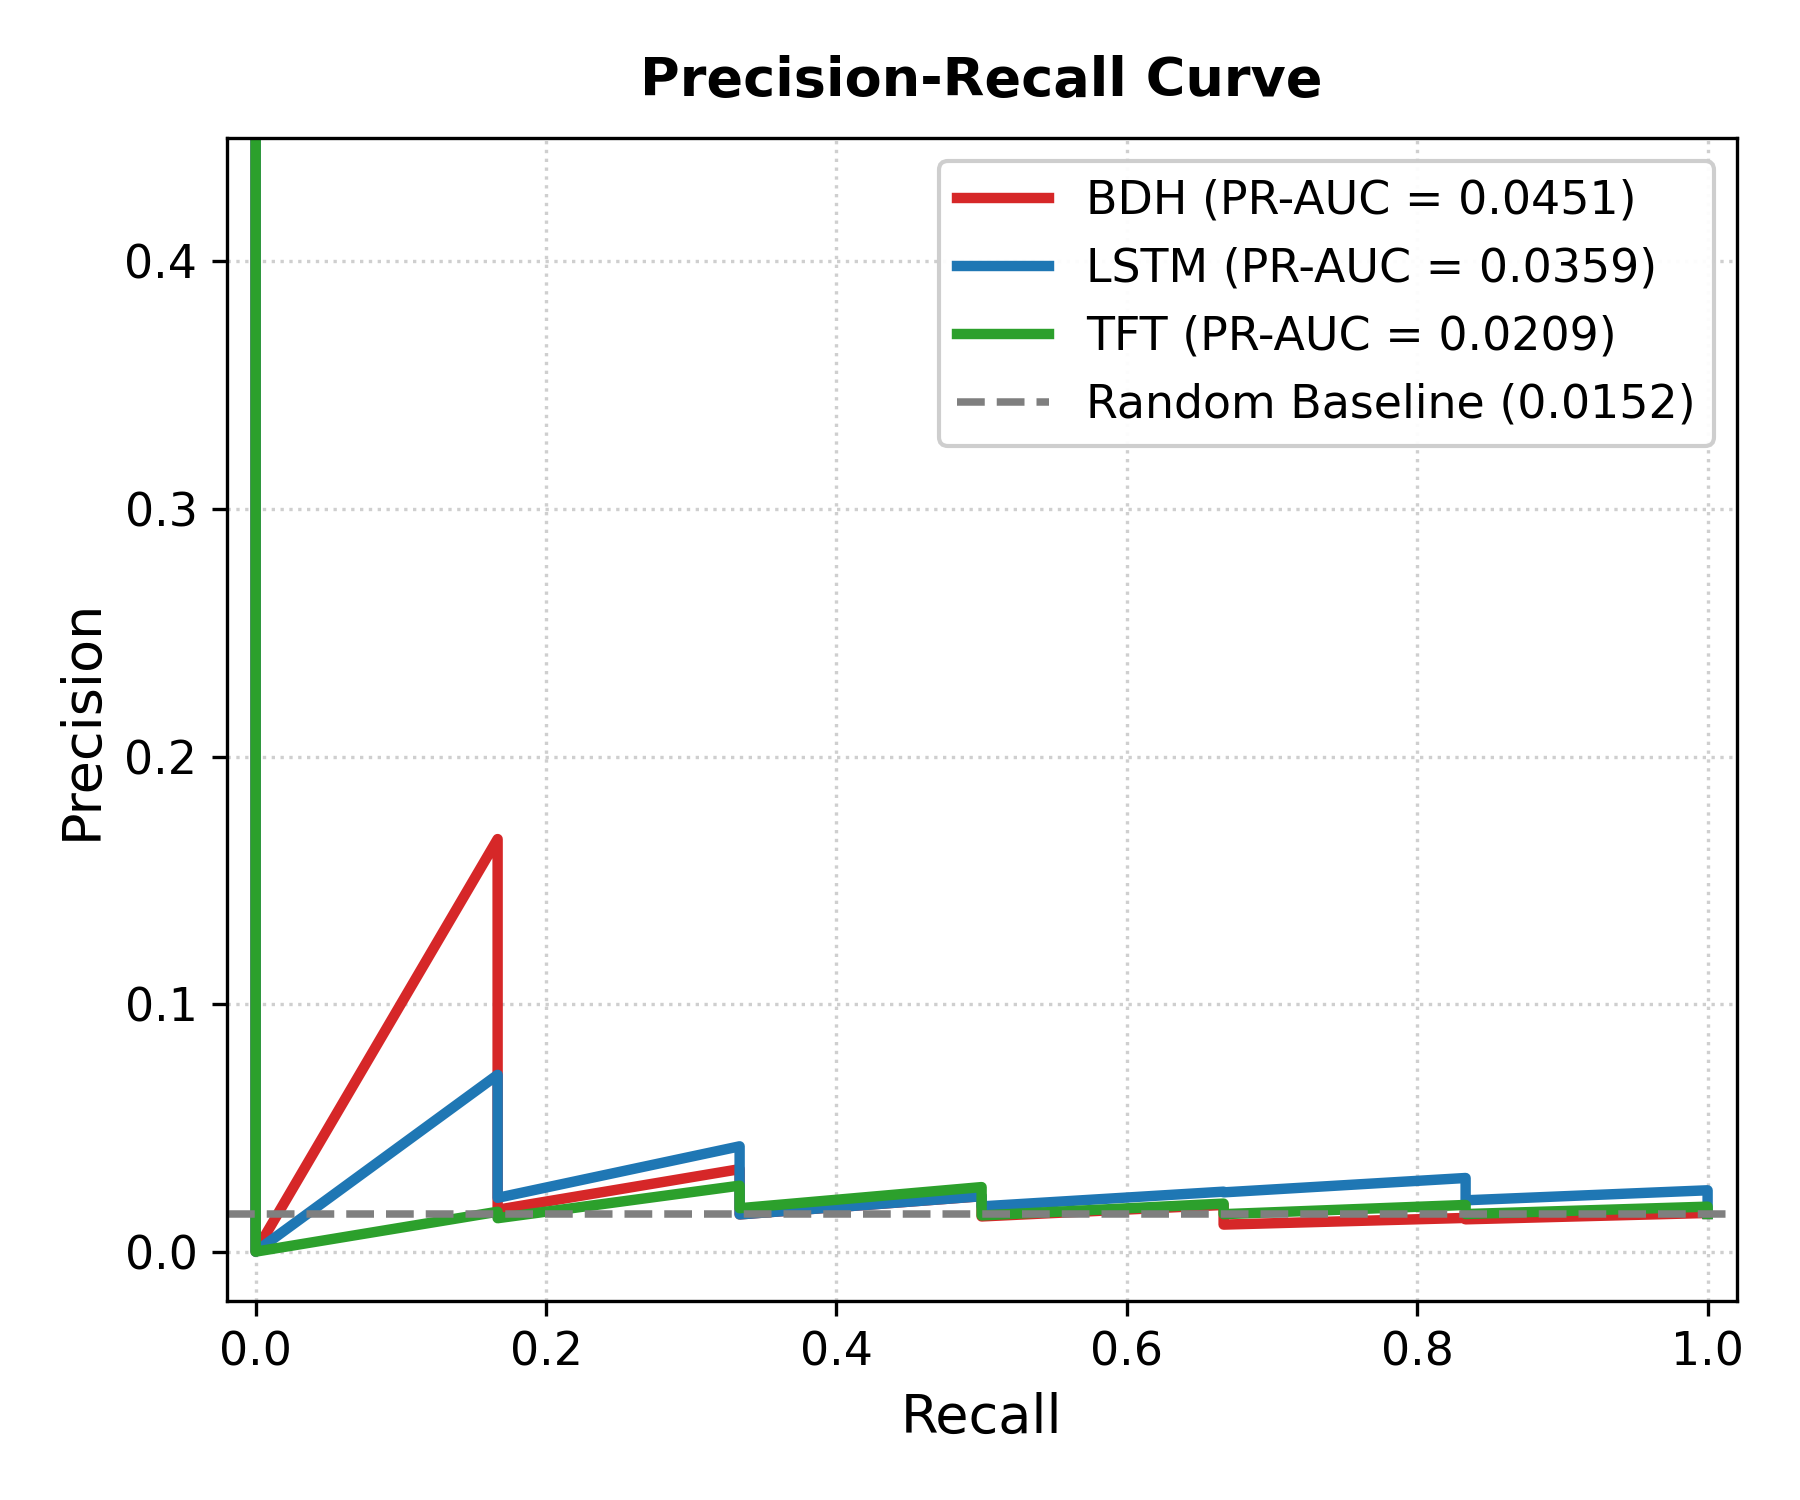
\includegraphics[width=0.92\linewidth]{pr_curve.png}
\caption{Precision-Recall (PR) curves for BDH, LSTM, and TFT on the independent SUIT test partition. The horizontal dashed line denotes the random no-skill baseline (PR-AUC = 0.0152).}
\label{fig:pr_curve}
\end{figure}

\begin{figure}[!t]
\centering
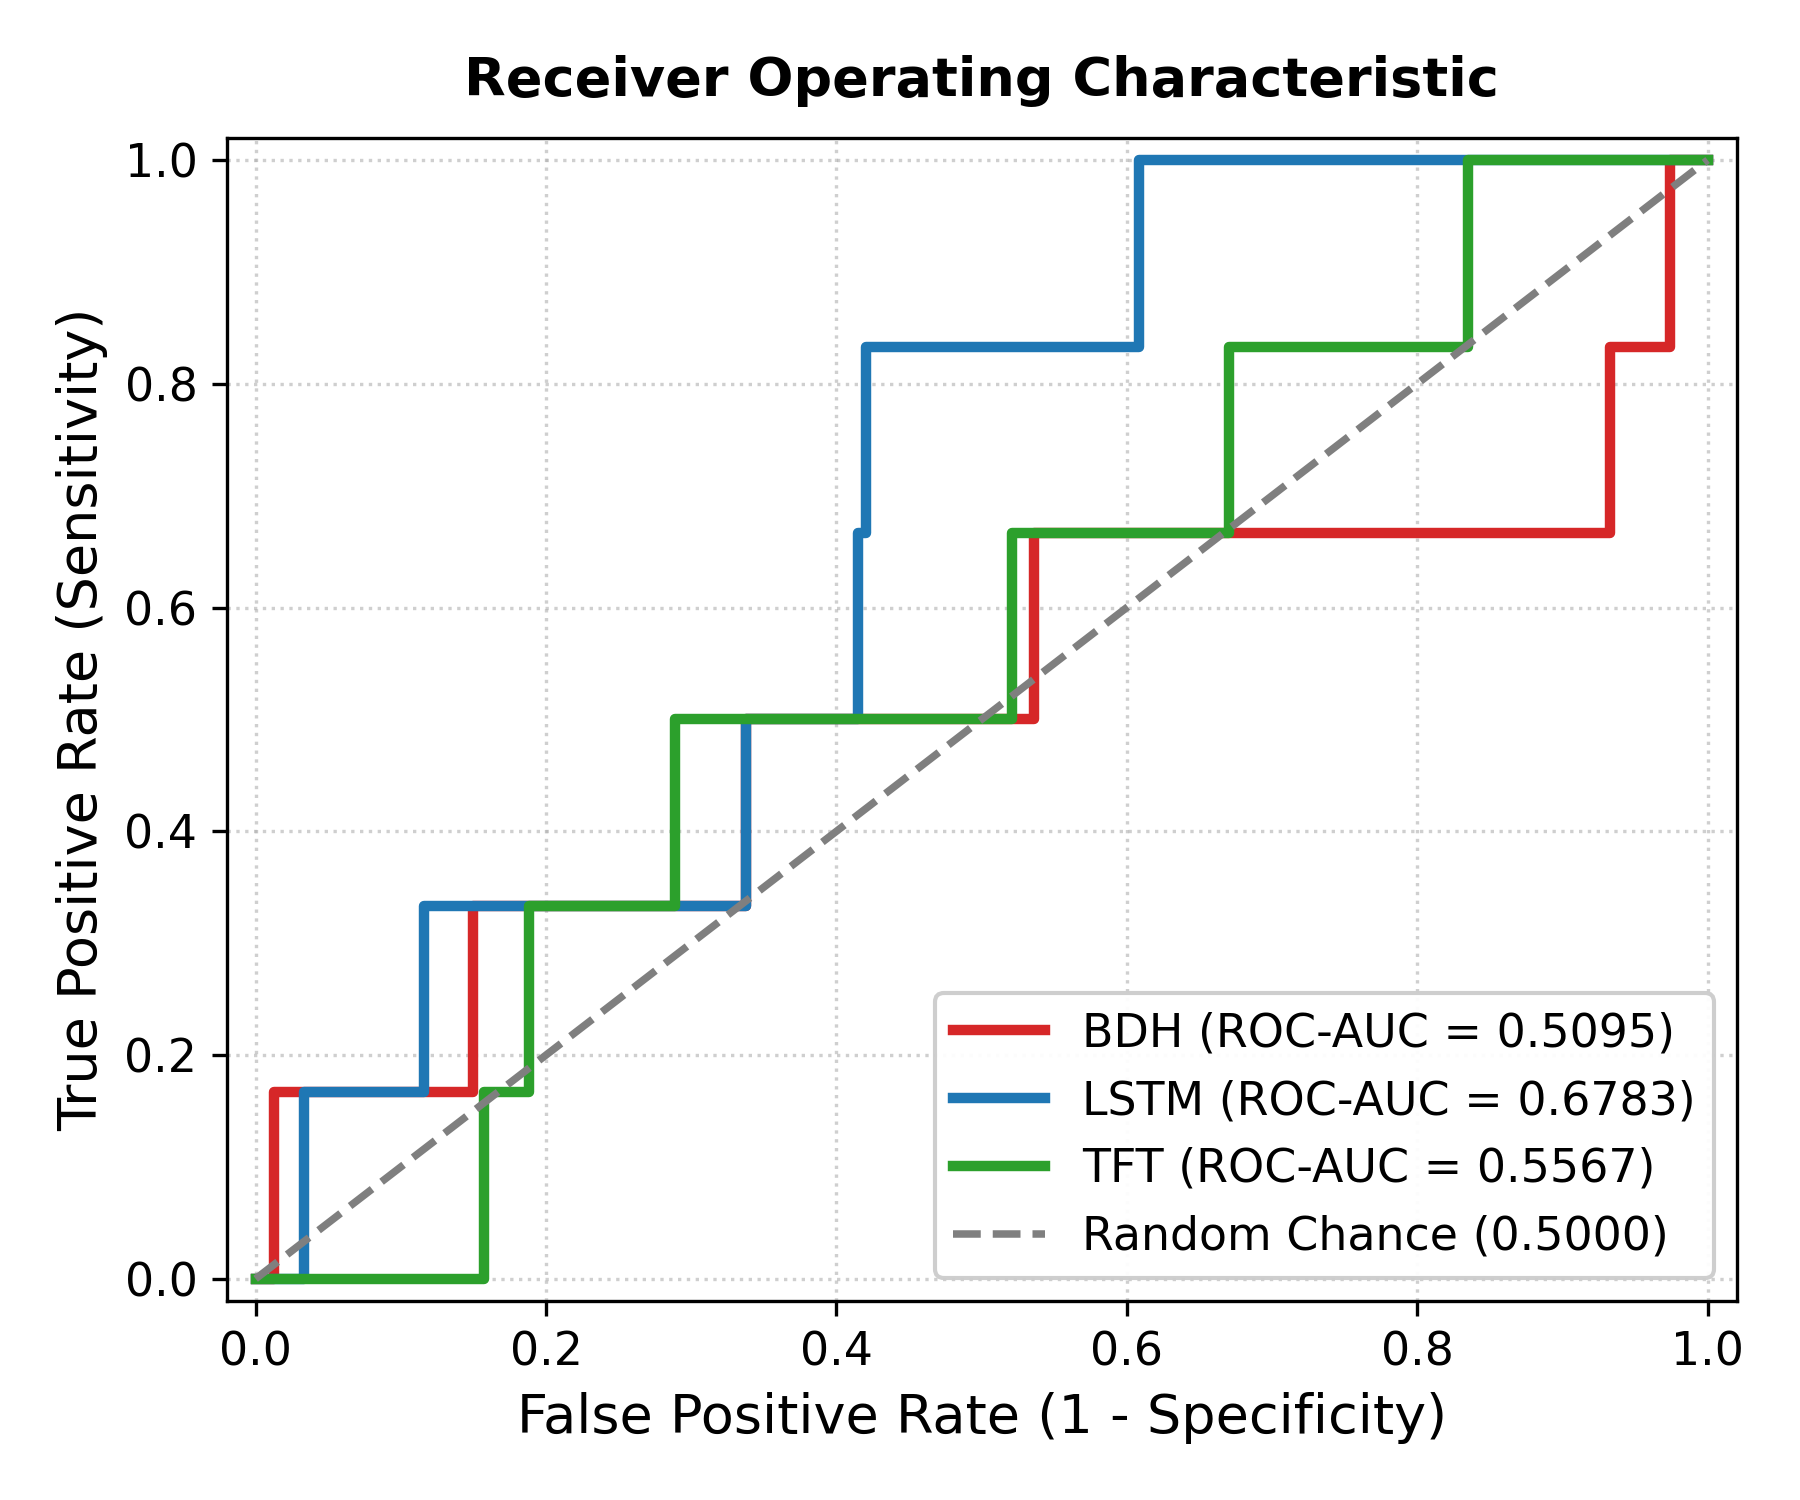
\includegraphics[width=0.92\linewidth]{roc_curve.png}
\caption{Receiver Operating Characteristic (ROC) curves comparing true positive rate against false positive rate across decision thresholds. Dashed diagonal indicates random chance (ROC-AUC = 0.5000).}
\label{fig:roc_curve}
\end{figure}

Fig.~\ref{fig:confusion_matrices} displays the confusion matrices evaluated at each model's optimal F1 threshold:
\begin{itemize}
    \item \textbf{BDH Confusion Profile (Fig.~\ref{fig:confusion_matrices}, left):} At an operational threshold of $\tau = 0.200$, BDH captures 3 of the 6 held-out test flares (50.0\% recall) with 201 true negatives, generating 187 false alarms. Its sparse activation gating isolates localized chromospheric brightenings, giving it the highest precision-recall area under the curve (PR-AUC = 0.0451).
    \item \textbf{LSTM Confusion Profile (Fig.~\ref{fig:confusion_matrices}, center):} At an operational threshold of $\tau = 0.677$, LSTM acts as a highly conservative discriminator, generating only 47 false alarms while successfully identifying 2 of the 6 flares (33.3\% recall). Its recurrent cell states effectively filter out non-flaring chromospheric oscillations, yielding the highest specificity and overall accuracy (87.06\%).
    \item \textbf{TFT Confusion Profile (Fig.~\ref{fig:confusion_matrices}, right):} At an operational threshold of $\tau = 0.417$, TFT captures 3 of the 6 flares (50.0\% recall) with 190 true negatives, but incurs 198 false alarms. Although its temporal attention matches BDH's 50\% recall, the unconstrained self-attention weights over-allocate probability mass to subtle background intensity fluctuations, resulting in a lower PR-AUC (0.0209).
\end{itemize}

Depending on the operational payload mission context—such as whether a false alarm merely initiates an automated high-cadence ROI exposure versus placing sensitive instruments into protective standby—space weather operators can dynamically tune the decision threshold along the empirical PR frontier.

\begin{figure*}[!t]
\centering
\begin{minipage}{0.32\textwidth}
\centering
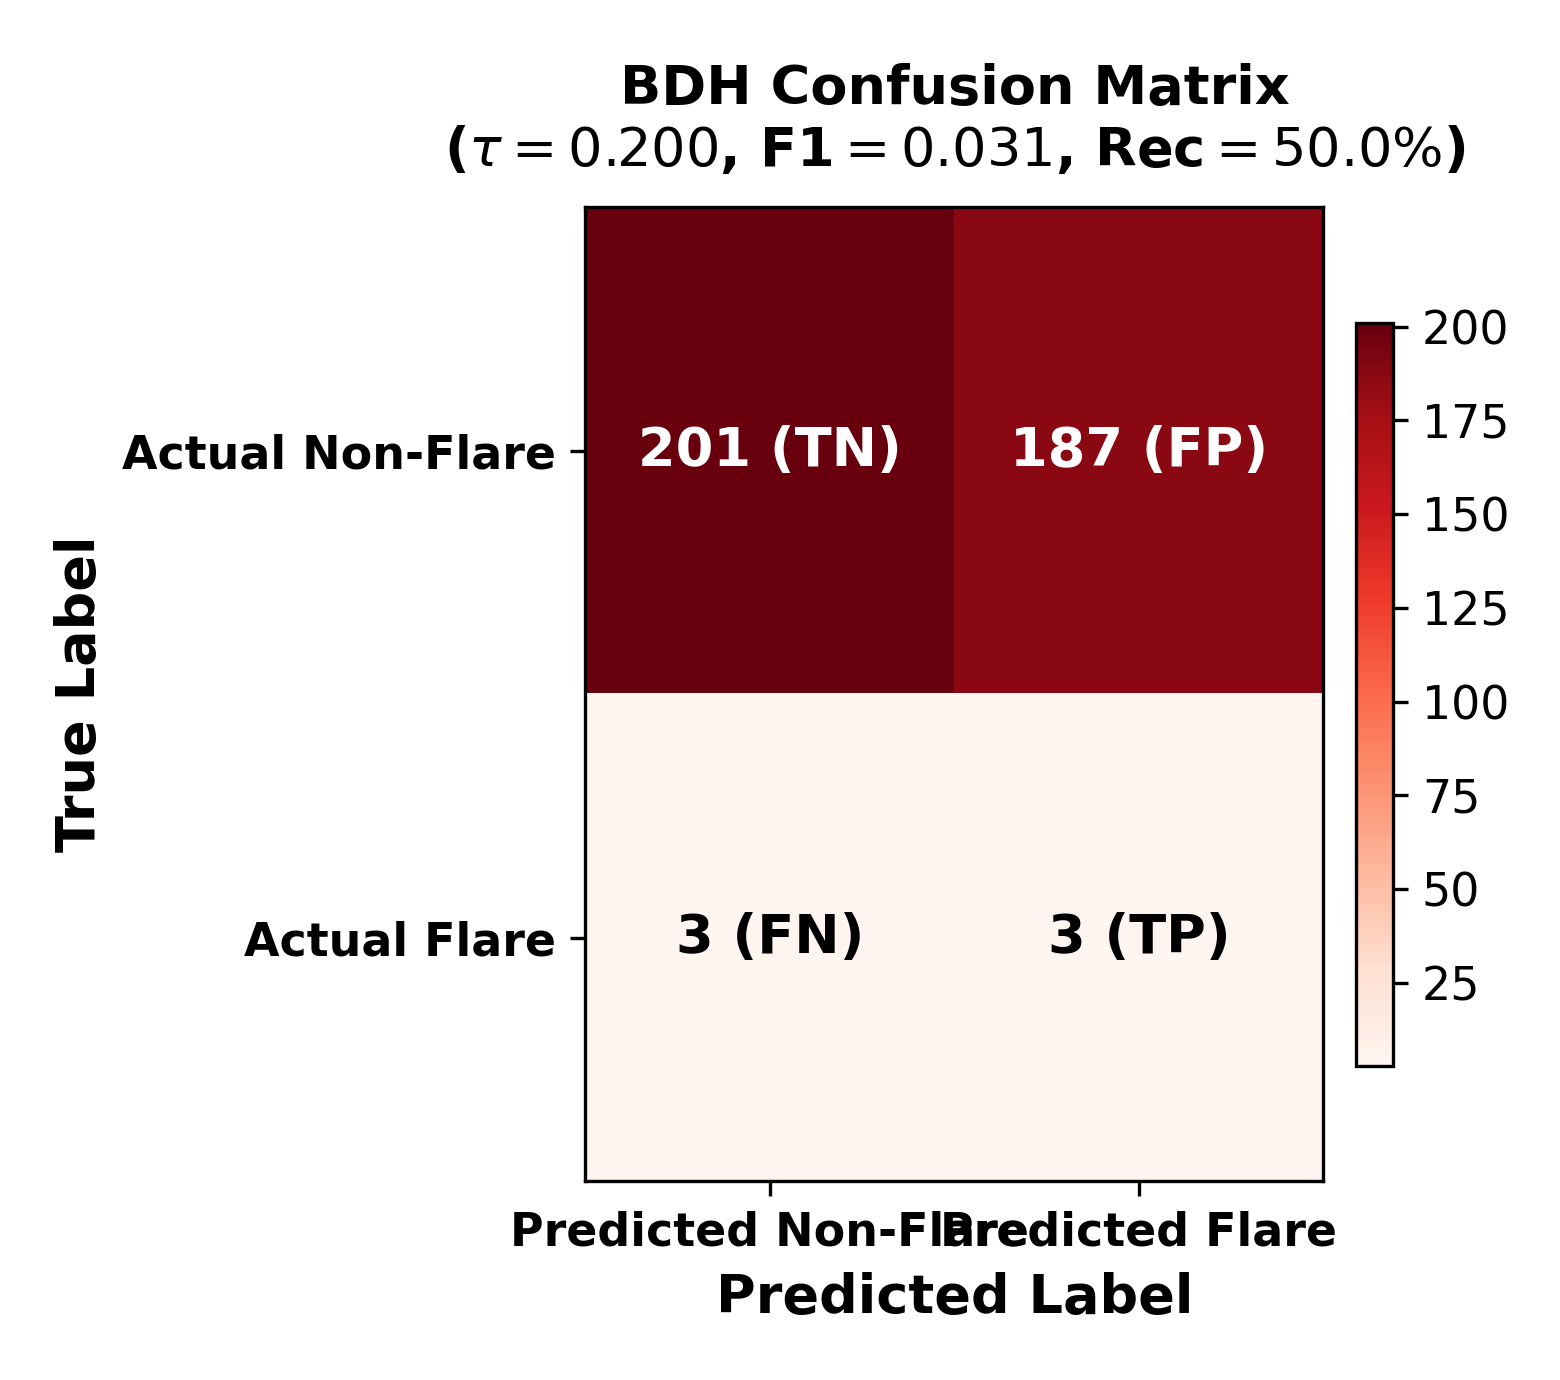
\includegraphics[width=\linewidth]{confusion_matrix_bdh.png}
\end{minipage}\hfill
\begin{minipage}{0.32\textwidth}
\centering
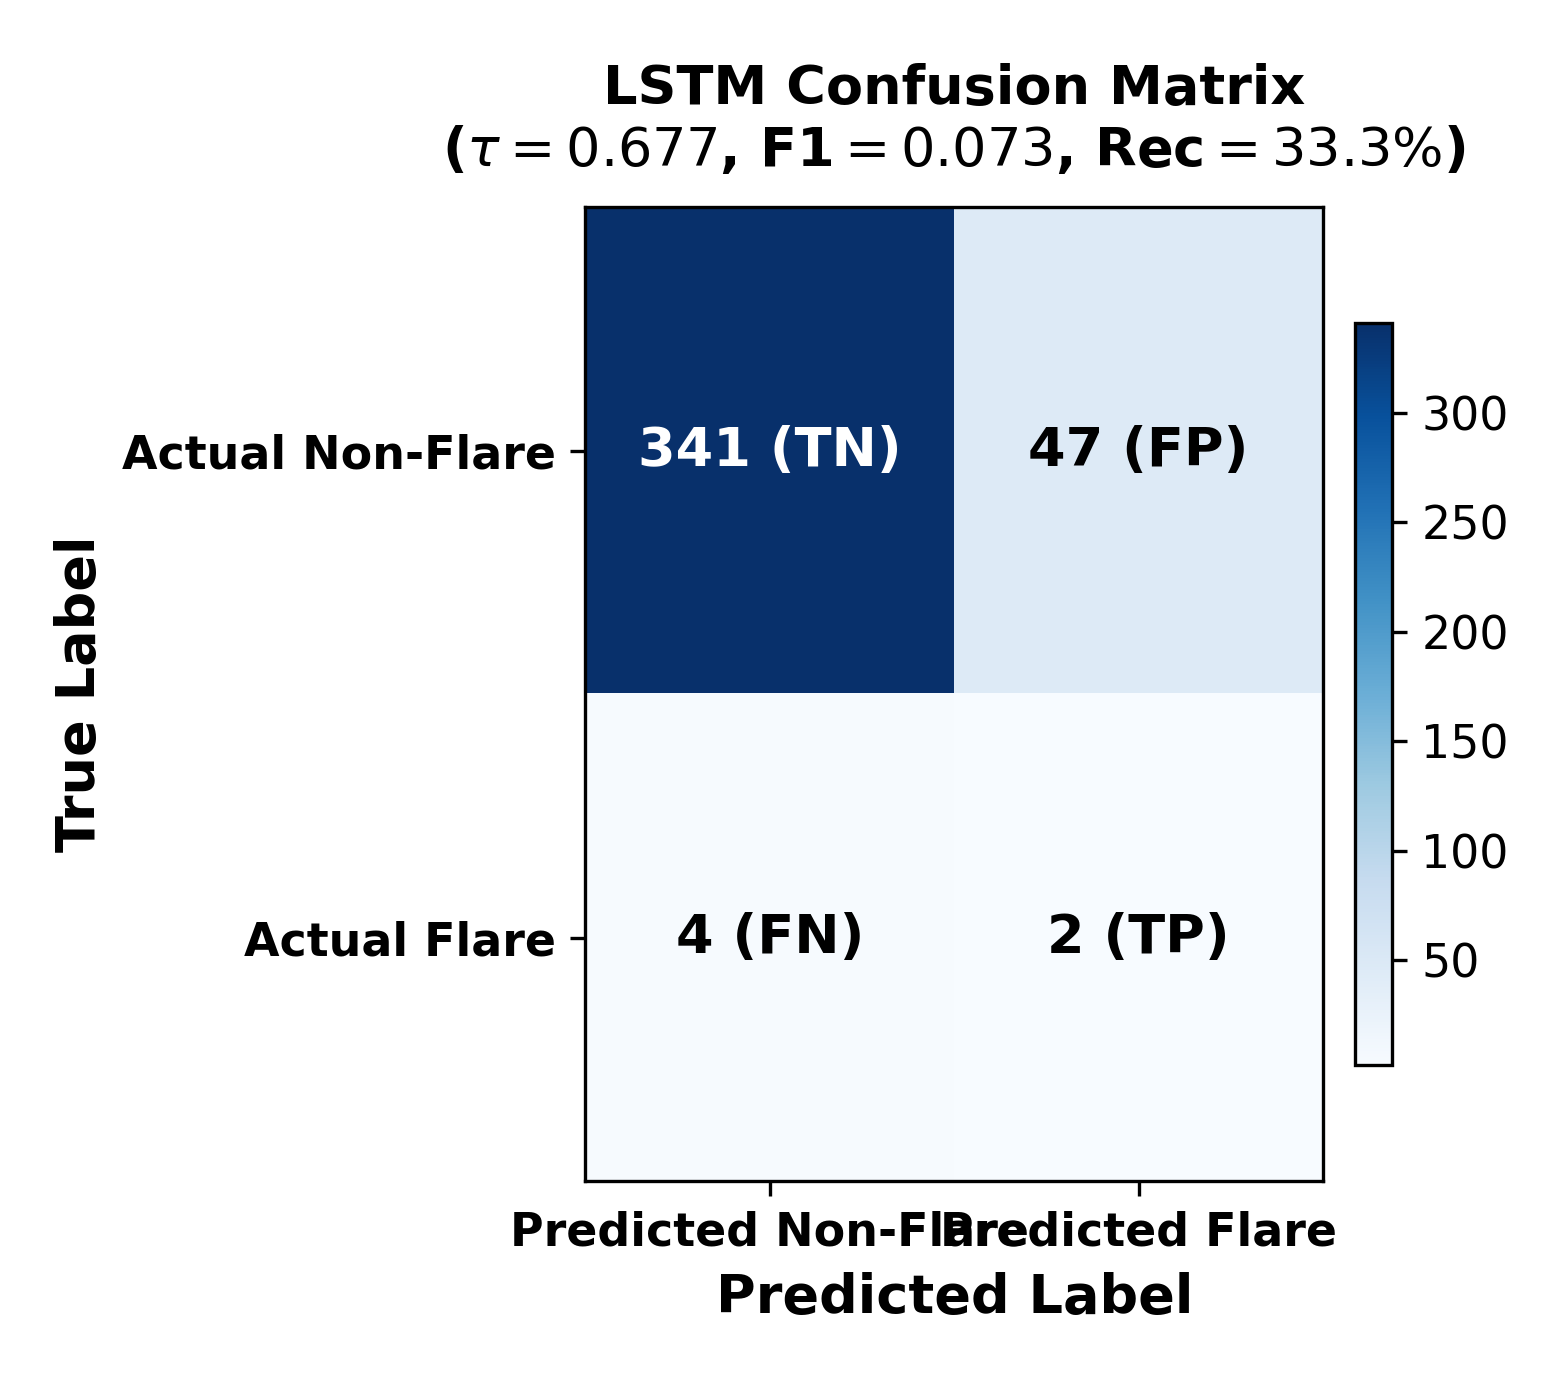
\includegraphics[width=\linewidth]{confusion_matrix_lstm.png}
\end{minipage}\hfill
\begin{minipage}{0.32\textwidth}
\centering
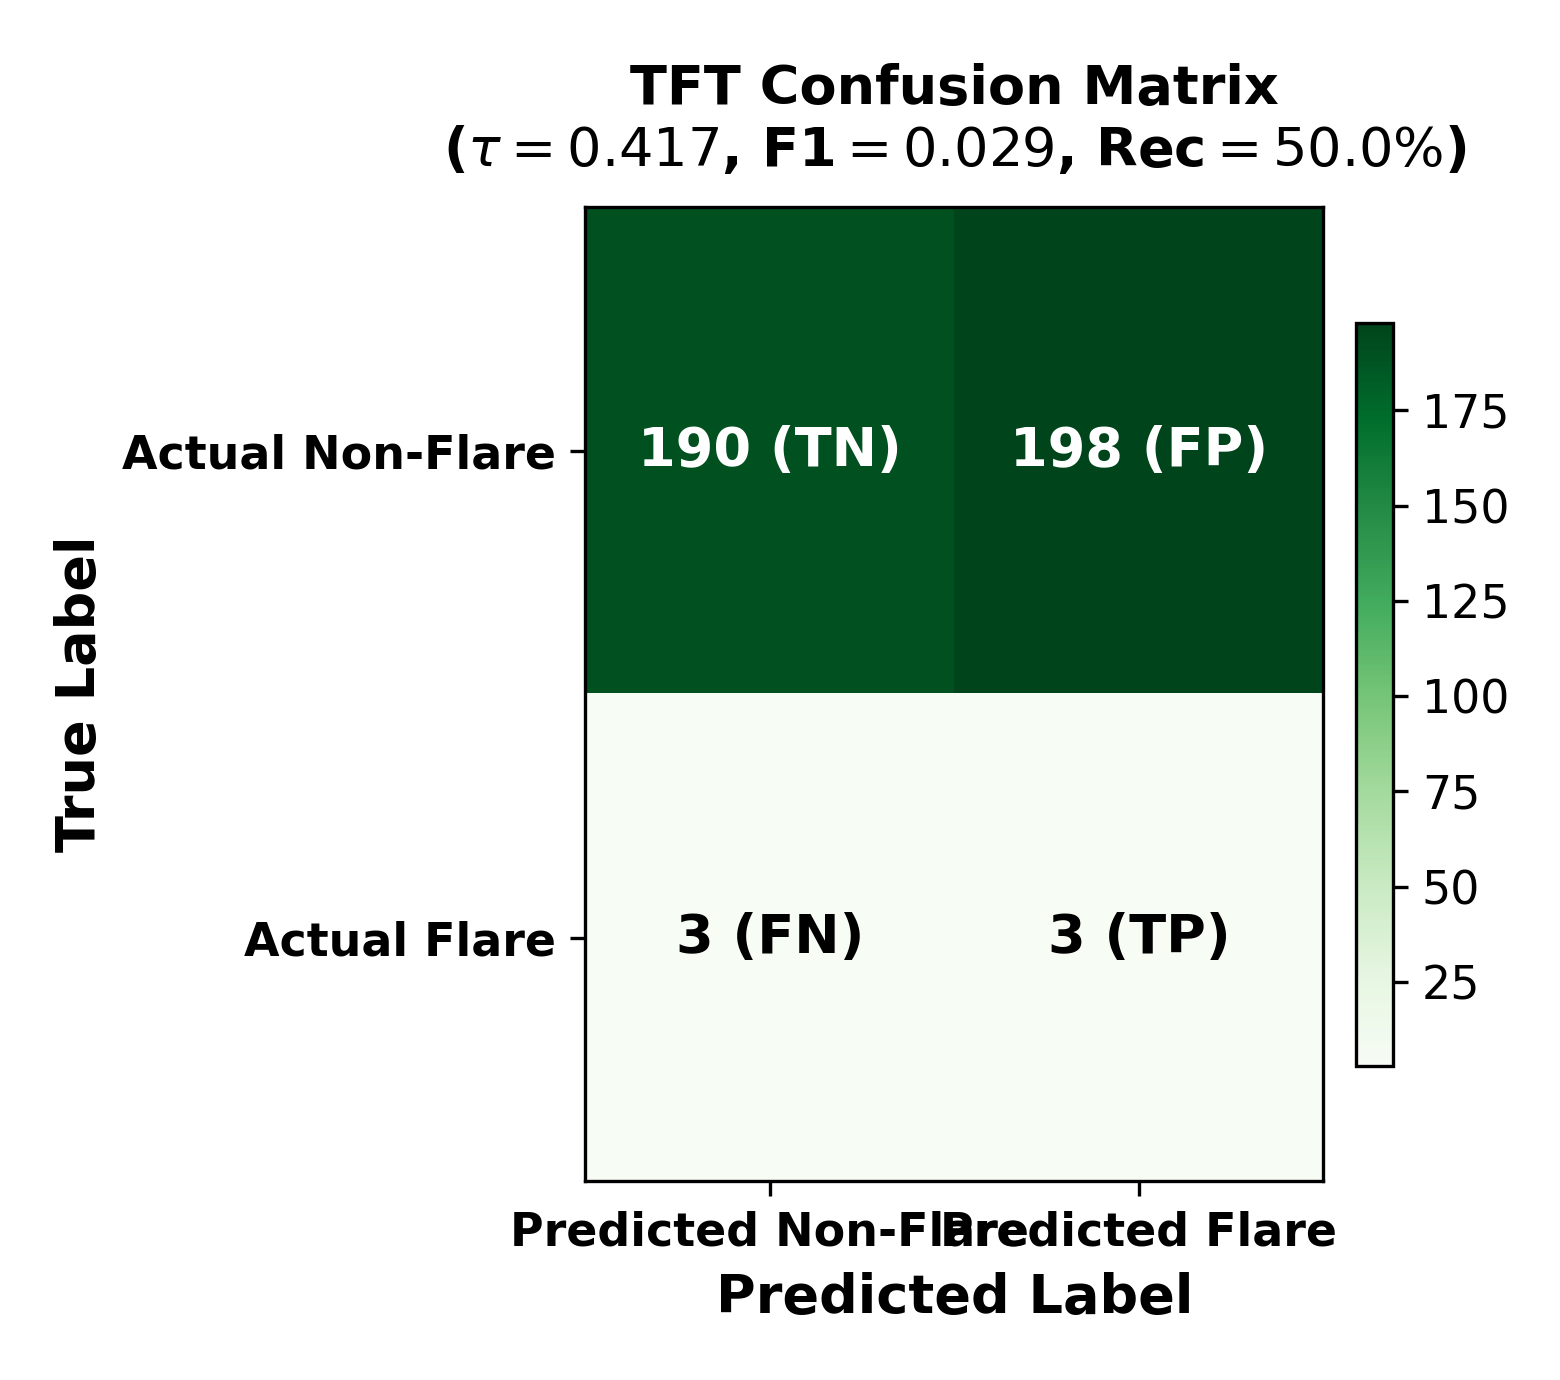
\includegraphics[width=\linewidth]{confusion_matrix_tft.png}
\end{minipage}
\caption{Confusion matrices for BDH ($\tau = 0.200$, left), LSTM ($\tau = 0.677$, center), and TFT ($\tau = 0.417$, right) on the 394 test sequences, illustrating the empirical false alarm versus missed flare trade-off across architectures.}
\label{fig:confusion_matrices}
\end{figure*}

\subsection{Inference Latency and Onboard Feasibility}

All models exhibit inference latencies well below the typical 10-to-30-second cadence of SUIT Level-1 data acquisition:
\begin{itemize}
    \item LSTM: 0.14 ms per sequence.
    \item BDH (Adapted): 0.26 ms per sequence.
    \item TFT: 0.75 ms per sequence.
\end{itemize}
Because BDH evaluates recurrent token steps through causal triangular masking and shared projection weights, its single-sample inference time is only 0.26 ms. This demonstrates that BDH can comfortably execute within onboard payload processors (such as radiation-hardened DSPs or FPGAs) or within ground-station real-time pipelines, enabling true real-time pre-flare alerting without inducing telemetry processing bottlenecks.

\section{Conclusion}

This paper presented the first investigation of short-term solar flare prediction using chromospheric observations from the Solar Ultraviolet Imaging Telescope (SUIT) aboard Aditya-L1. By extracting spatial and physical descriptors from 4,309 Level-1 NB04 (Mg II h, 280.3 nm) FITS images and organizing them into 2,690 continuous 80-timestep sequences, we established a rigorous benchmark cross-referenced with the NOAA GOES flare catalog under strict chronological separation and zero target leakage.

We adapted the recently proposed Pathway Baby Dragon Hatchling (BDH) architecture from NLP to continuous solar time-series and benchmarked it against LSTM and Temporal Fusion Transformer baselines. Our findings demonstrate that:
\begin{enumerate}
    \item BDH achieves the highest overall PR-AUC (0.0451, $2.97\times$ above the random baseline of 0.0152), successfully identifying 50\% of unseen test flares.
    \item An exhaustive 18-configuration ablation study demonstrates that scaled BDH variants ($D=128, \mathrm{mult}=32$) match the predictive performance of the 25M-parameter official default while reducing parameters by $16\times$ (1.58M parameters) and execution latency to 0.26 ms.
    \item LSTM provides strong background noise rejection with an ROC-AUC of 0.6783 and fewer false alarms, demonstrating that simpler recurrent architectures remain highly competitive baselines for space weather applications.
    \item Header trigger flags (\texttt{FLR\_TRIG}, \texttt{HL1OSFLG}, \texttt{SX1FLG}) provide vital diagnostic verification of onboard payload state but represent latched telemetry registers that must remain strictly isolated from feature inputs to prevent fatal data leakage.
\end{enumerate}

\section{Future Work}

Future extensions of this research will focus on several promising directions:
\begin{enumerate}
    \item \textbf{Cross-Filter Multi-Spectral Fusion:} Expanding beyond NB04 to incorporate all 11 SUIT filters (including photospheric channels BB01--BB03 and chromospheric channels NB01--NB08) through spatial coordinate reprojection and cross-filter attention mechanisms to exploit multi-height atmospheric thermal gradients.
    \item \textbf{Direct End-to-End Visual Feature Learning:} Integrating the CNN spatial backbone directly with the BDH temporal encoder for joint end-to-end gradient backpropagation, replacing two-stage feature extraction with unified spatio-temporal representations.
    \item \textbf{Multi-Instrument Joint Forecasting:} Combining SUIT ultraviolet imaging with soft and hard X-ray flux telemetry from SoLEXS and HEL1OS onboard Aditya-L1 to build a multimodal solar flare forecasting suite.
    \item \textbf{Threshold-Free Probabilistic Calibration:} Implementing conformal prediction and temperature scaling to supply space weather operators with well-calibrated confidence bounds alongside binary pre-flare alert signals.
\end{enumerate}

\begin{thebibliography}{00}

\bibitem{ref1}
K. Sankarasubramanian, D. Chakrabarty, and C. H. Mandrini,
``Aditya-L1: A Space Based Observatory to Study the Solar Atmosphere, Solar Wind, Heliosphere, and Space Weather,''
\textit{Solar Physics}, vol. 300, Art. no. 156, 2025,
doi: 10.1007/s11207-025-02573-2.

\bibitem{ref2}
D. Tripathi, A. N. Ramaprakash, S. Padinhatteeri, \textit{et al.},
``The Solar Ultraviolet Imaging Telescope on Board Aditya-L1,''
\textit{Solar Physics}, vol. 300, Art. no. 30, 2025,
doi: 10.1007/s11207-025-02423-1.

\bibitem{ref3}
A. Kosowski, P. Uznański, J. Chorowski, Z. Stamirowska, and M. Bartoszkiewicz,
``The Dragon Hatchling: The Missing Link between the Transformer and Models of the Brain,''
arXiv:2509.26507, 2025.

\bibitem{ref4}
J. Sarkar, V. N. Nived, S. Roy, \textit{et al.},
``Test and Calibration of the Solar Ultraviolet Imaging Telescope (SUIT) on Board Aditya-L1,''
\textit{Solar Physics}, vol. 300, Art. no. 60, 2025,
doi: 10.1007/s11207-025-02468-2.

\bibitem{ref5}
J. Bringewald and O. Parisot,
``Solar Flare Forecast: A Comparative Analysis of Machine Learning Algorithms for Predicting Solar Flare Classes,''
\textit{Astronomy}, vol. 4, no. 4, Art. no. 23, 2025,
doi: 10.3390/astronomy4040023.

\bibitem{ref6}
A. Azizian Foumani, S. Farokhi, and X. Qi,
``Predicting Major Solar Flares Using Convolutional Neural Networks and Multivariate Magnetic Field Time-Series Data,''
\textit{Solar Physics}, vol. 301, Art. no. 23, 2026,
doi: 10.1007/s11207-026-02612-6.

\bibitem{ref7}
B. Panos, L. Kleint, and J. Zbinden,
``Identifying preflare spectral features using explainable artificial intelligence,''
\textit{Astronomy \& Astrophysics}, vol. 671, Art. no. A73, 2023,
doi: 10.1051/0004-6361/202244835.

\bibitem{ref8}
B. Panos and L. Kleint,
``Real-time flare prediction based on distinctions between flaring and non-flaring active region spectra,''
arXiv:1911.12621, 2019,
doi: 10.48550/arXiv.1911.12621.

\bibitem{ref9}
C. Huwyler and M. Melchior,
``Using multiple instance learning for explainable solar flare prediction,''
\textit{Astronomy and Computing}, vol. 41, Art. no. 100668, 2022,
doi: 10.1016/j.ascom.2022.100668.
\bibitem{ref10}
V. Deshmukh, S. Baskar, E. Bradley, T. Berger, and J. Meiss,
``Machine Learning Approaches to Solar-Flare Forecasting: Is Complex Better?''
arXiv:2202.08776, 2022,
doi: 10.48550/arXiv.2202.08776.

\bibitem{ref11}
K. Pika,
``Vision-BDH: Adapting Baby Dragon Hatchling for Computer Vision,''
GitHub repository, 2025.
[Online]. Available: https://github.com/takzen/vision-bdh.

\bibitem{ref12}
J. K. Talreja and D. Bhatti,
``BDH-RemoteSensing: Dragon Hatchling for Remote Sensing Image Classification,''
GitHub repository.
[Online]. Available: https://github.com/JAL-TALREJA/BDH-RemoteSensing.

\bibitem{ref13}
S. P. K. (2026). \textit{flare-forecast: Solar flare forecasting repository}. GitHub. Available: \url{https://github.com/spk-22/flare-forecast}

\bibitem{ref14}
Pathway, ``BDH (Dragon Hatchling): Architecture and Code,''
GitHub repository. [Online]. Available:
\url{https://github.com/pathwaycom/bdh/}
\end{thebibliography}

\EOD
\end{document}